\section{Additional results}
\label{app:results}

\subsection{Main result: supporting results}
the learning curves of the autoregressive reference (Appendix~\ref{app:ar_curves}), \methodGRPO{} read under both samplers (Appendix~\ref{app:grpo_chain}), and the recipe of the masked-diffusion reference (Appendix~\ref{app:d1}).

\subsubsection{Autoregressive reference: learning curves}
\label{app:ar_curves}
Table~\ref{tab:ar_curves} gives the curves behind the GPT-2 rows of Table~\ref{tab:main}: the supervised stage by epoch and token-level GRPO/PPO by iteration. Token-level RL climbs steadily on Countdown and Game24, much of it within the first 100 iterations; on K\&K, where the supervised policy is already sharp, it holds; on Sudoku, where the supervised model solves about one puzzle in a hundred, the reward is too sparse to move it. The autoregressive policy sees the same problems and verifier as the flow policies and at least as many rollouts per iteration; what differs is the action space the estimator acts on.

\begin{table}[H]\centering\small
\caption{AR control (GPT-2, 124M), held-out accuracy (\%) with greedy decoding. Top: supervised fine-tuning by epoch (Sudoku: epochs 2, 4, \dots, 20, scored by the SFT script's solved-grid metric; the verifier gives 1.2 at epoch 20). Bottom: token-level GRPO/PPO by iteration (32 prompts $\times$ 8 samples per iteration). Bold: the highest cell of each row.}\label{tab:ar_curves}
\resizebox{\linewidth}{!}{%
\begin{tabular}{@{}lcccccccccc@{}}\toprule
SFT epoch & 1 & 2 & 3 & 4 & 5 & 6 & 7 & 8 & 9 & 10\\\midrule
Countdown & 26.5 & 30.8 & 38.1 & 38.8 & 41.1 & 43.9 & 42.4 & \textbf{44.2} & 43.6 & 42.8\\
Sudoku (epochs 2--20) & \phantom{0}0.6 & \phantom{0}0.9 & \phantom{0}1.1 & \phantom{0}1.3 & \phantom{0}1.3 & \phantom{0}1.4 & \phantom{0}1.4 & \phantom{0}1.4 & \textbf{\phantom{0}1.7} & \phantom{0}1.7\\
K\&K & 28.2 & 46.6 & 68.7 & 82.8 & 87.1 & 88.5 & 91.4 & 92.3 & 92.8 & \textbf{92.9}\\
Game24 (init.\ from the Countdown model) & 19.6 & \textbf{26.9} & 22.1 & 21.3 & 19.9 & 21.7 & 21.0 & 20.8 & 20.7 & 21.6\\
Game24 (init.\ from vanilla GPT-2) & \phantom{0}1.1 & \phantom{0}9.8 & 11.4 & \textbf{12.4} & \phantom{0}9.0 & \phantom{0}9.5 & 10.3 & 11.2 & \phantom{0}9.7 & \phantom{0}9.7\\
\midrule
RL iteration & 0 & 100 & 150 & 200 & 300 & 400 & 500 & 550 & 600 & \\\midrule
Countdown, $10^{-5}$ & 44.2 & 52.3 & 55.2 & 54.8 & 57.8 & 59.0 & 60.6 & 61.3 & \textbf{61.7} & \\
Sudoku, $10^{-5}$ & \phantom{0}1.2 & \phantom{0}1.1 & \phantom{0}1.4 & \textbf{\phantom{0}1.6} & \phantom{0}1.6 & \phantom{0}1.5 & \phantom{0}1.6 & \phantom{0}1.4 & \phantom{0}1.6 & \\
K\&K, $3\times10^{-6}$ & 92.9 & 93.0 & \textbf{93.2} & 93.1 & 92.9 & 92.8 & 92.7 & 92.8 & 92.7 & \\
Game24, $10^{-5}$ & 26.9 & 39.8 & 40.2 & 42.5 & 45.8 & 44.2 & 42.8 & \textbf{46.2} & 46.0 & \\
\bottomrule\end{tabular}}\end{table}

\subsubsection{\methodGRPO{} under its own sampler and under the deployment sampler}
\label{app:grpo_chain}
\methodGRPO{} is trained under the 16-step $\gamma4$@16 sampler (the cheap sampler except on Sudoku) and, like every row of Table~\ref{tab:main}, read under the deployment sampler. Two checks show that this mismatch is not what limits it. Read under its own sampler, the Countdown runs gain about one point over the base. Trained under the deployment sampler instead, with the same recipe otherwise, \methodGRPO{} gains $+0.1$ on Countdown and $+3.5$ on Game24. The estimator gains little under either sampler.

\subsubsection{The masked-diffusion reference: d1 on our tasks}
\label{app:d1}
d1 \citep{zhao2025d1} is the most used RL recipe for masked diffusion language models: LLaDA-8B-Instruct \citep{nie2025llada} with LoRA, a supervised stage, and diffu-GRPO, a GRPO variant whose per-token log-probabilities come from one forward pass in which all completion tokens are masked. That estimator requires a mask token and a discrete masked-diffusion model, so it cannot be applied to a continuous flow model; \methodGRPO{} is its counterpart on ELF. We ran d1's own recipe, unchanged, on its own base model and on our four held-out sets, with the authors' code and hyperparameters (LoRA rank 128 on all attention and MLP projections, six generations per prompt, 256-token completions with 128 diffusion steps, block length 32, learning rate $3\times10^{-6}$, 12 inner iterations, KL weight 0.04, clip $0.5$), prompts and rewards in d1's own formats, and accuracy as our exact-success metric. The supervised stage is completion-only masked SFT on the same training data as ELF-B's task SFT (3--20 epochs per task); diffu-GRPO then runs from the merged SFT model for 8{,}000 inner steps, about 32k rollouts, the budget of our pathwise runs. The comparison is across architectures and training histories: LLaDA-8B-Instruct was never trained on these tasks and its supervised stage is a LoRA run, whereas ELF-B is trained in full, so we make no claim about the ceiling of masked diffusion models. What Table~\ref{tab:main} shows is the behaviour of the estimator: diffu-GRPO moves the supervised model by under three points on every task, consistent with d1's own results on its easier three-number Countdown and $4{\times}4$ Sudoku.

% ---- CUT 2026-09-26 (not needed for the main narrative): Choice of the Game24 base checkpoint ----
\iffalse
\subsubsection{Choice of the Game24 base checkpoint}
\label{app:g24_sft}
Game24 is the one task on which more supervised training hurts, so the base checkpoint is chosen on held-out accuracy (Table~\ref{tab:g24_sft}): the model is still improving at epoch 10, peaks at epoch 20 and declines afterwards under every sampler, the SDE samplers first and the ODE sampler from epoch 30. All Game24 RL and loop runs start from the epoch-20 checkpoint (45.0 at $\gamma56$@64). The decline is a memorisation effect of the set-split: the training orderings of a held-out set never appear, but the training derivations do, and late SFT epochs fit them at the expense of the arithmetic generalisation the verifier rewards.

\begin{table}[H]\centering\small
\caption{Game24 held-out (set-split) accuracy of the SFT model by epoch and sampler; bold: the best epoch per sampler.}\label{tab:g24_sft}
\begin{tabular}{@{}lccccccc@{}}\toprule
epoch & 4 & 6 & 8 & 10 & \textbf{20} & 30 & 40\\\midrule
ODE-64 & 3.7 & 26.0 & 28.2 & 29.9 & \textbf{35.2} & 35.2 & 30.5\\
$\gamma4$@16 & 9.7 & 28.0 & 29.8 & 32.5 & \textbf{35.4} & 32.3 & 29.8\\
$\gamma28$@32 & 3.6 & 35.3 & 36.1 & 37.9 & \textbf{42.6} & 38.7 & 32.1\\
$\gamma56$@64 & 4.2 & 37.4 & 41.0 & 42.8 & \textbf{45.0} & 39.8 & 34.7\\\bottomrule\end{tabular}\end{table}

\fi


% ---- CUT 2026-09-26 (not needed for the main narrative): Knights-and-Knaves by number of people ----
\iffalse
\subsubsection{Knights-and-Knaves by number of people}
\label{app:kk_by_n}
Table~\ref{tab:kk_by_n} splits K\&K accuracy by the number of people in the puzzle. The base model is near-perfect on 4-person puzzles and weakest on 6-person ones; \methodGRPO{} improves all sizes by similar absolute amounts; the early \methodSVGTwoD{} checkpoint shown (250 iterations, before the run reaches the level of Table~\ref{tab:main}) has moved the 4- and 5-person puzzles but not yet the 6-person ones; the fresh-problem loop closes the remaining gap on 6-person puzzles ($51.8\to97.6$), within 1.4 points of the gold-supervised model (99.0) without ever seeing a gold label.

\begin{table}[H]\centering\small
\caption{K\&K held-out accuracy by number of people (deployment sampler $\gamma56$@64; ODE-64 in parentheses for the SFT and loop rows).}\label{tab:kk_by_n}
\begin{tabular}{@{}lcccc@{}}\toprule
model & all & 4 people & 5 people & 6 people\\\midrule
SFT epoch 4 (base) & 67.5 (57.8) & 86.8 (80.8) & 63.5 (57.9) & 51.8 (34.2)\\
GRPO (600 iterations) & 74.6 & 92.7 & 72.6 & 58.2\\
\methodSVGTwoD{} (250 iterations) & 70.3 & 92.1 & 68.6 & 50.0\\
fresh-problem loop, round 5 (Table~\ref{tab:loop}) & 99.1 (96.0) & 100.0 (100.0) & 99.7 (97.7) & 97.6 (90.1)\\
gold SFT epoch 6 & 95.4 (88.8) & 99.9 (99.9) & 96.8 (91.8) & 89.6 (74.8)\\
gold SFT epoch 8 & 99.7 (96.8) & 100.0 (100.0) & 100.0 (98.5) & 99.0 (91.8)\\\bottomrule\end{tabular}\end{table}

\fi


% ---- CUT 2026-09-26 (not needed for the main narrative): What the policy gradient changes: failure modes and examples ----
\iffalse
\subsubsection{What the policy gradient changes: failure modes and examples}
\label{app:failure_modes}
The Countdown and Game24 verifiers accept a derivation only if every equation is arithmetically exact, every operand is an input number or an earlier result used at most once, and the last result equals the target. Table~\ref{tab:failure_modes} classifies every held-out sample by the first rule it violates (our classifier reproduces the verifier's accept/reject decision exactly). Two facts stand out. No sample ever misses the target: the models always \emph{write} the target as the last result, so a wrong derivation always fails upstream, almost always by one arithmetically false equation. () What RL changes is therefore the rate of arithmetically false equations: from $47.8\%$ to $31.5\%$ of samples on Game24 and from $52.2\%$ to $41.4\%$ on Countdown, while the rate of number-use violations stays at $5$--$10\%$ (the pathwise update raises it slightly on Game24, the loop lowers it again). Table~\ref{tab:examples} shows held-out problems on which the base and the pathwise policy disagree: on Game24 the pathwise policy fixes $340$ problems and breaks $135$ relative to the base ($+12.8$ net); on Countdown $408$ and $228$ ($+9.0$ net).

\begin{table}[H]\centering\small
\caption{Failure-mode breakdown of held-out samples at the deployment sampler (\% of samples; ``arithmetic'' = at least one false equation; ``number use'' = an operand that is not available; ``format'' = unparsable). No sample in any run ends on a result different from the target.}\label{tab:failure_modes}
\begin{tabular}{@{}llcccc@{}}\toprule
task & policy & correct & arithmetic & number use & format\\\midrule
Game24 & SFT base & 45.0 & 47.8 & 7.2 & 0.0\\
 & GRPO (400) & 48.1 & 44.9 & 7.0 & 0.0\\
 & \methodSVGTwoD{} (1000) & 57.8 & 31.5 & 10.4 & 0.3\\
 & loop round 4 & 57.7 & 36.2 & 6.0 & 0.1\\\midrule
Countdown & SFT base & 42.2 & 52.2 & 5.5 & 0.1\\
 & \methodSVGScalar{} (1000) & 51.2 & 41.4 & 6.3 & 1.0\\
 & loop round 4 & 54.4 & 40.5 & 5.0 & 0.1\\\bottomrule\end{tabular}\end{table}

\begin{table}[H]\centering\scriptsize
\caption{Held-out examples (deployment sampler). \checkmark/\texttimes: verifier verdict. The Game24 gold derivation is one of several valid ones; the models are not asked to reproduce it.}\label{tab:examples}
\resizebox{\linewidth}{!}{%
\begin{tabular}{@{}llll@{}}\toprule
problem & SFT base & pathwise policy & \\\midrule
\multicolumn{4}{@{}l}{\emph{Game24 (base 45.0, \methodSVGTwoD{} 57.8)}}\\
2 2 9 8 $\to$ 24 & 8+2=10, 9*2=18, 18+10=24 \texttimes & 8$-$2=6, 2*9=18, 6+18=24 \checkmark & base: false equation\\
2 2 4 6 $\to$ 24 & 2*2=4, 4*4=18, 6+18=24 \texttimes & 4/2=2, 2+2=4, 4*6=24 \checkmark & base: false equation\\
13 4 12 7 $\to$ 24 & 4+13=17, 17*12=168, 168/7=24 \texttimes & 13$-$4=9, 9$-$7=2, 2*12=24 \checkmark & base: false division\\
5 9 4 6 $\to$ 24 & 9+6=15, 15+4=19, 19+5=24 \checkmark & 9$-$5=4, 6$-$4=6, 6*4=24 \texttimes & pathwise: false equation\\
6 11 6 6 $\to$ 24 & 11*6=66, 6*6=36, 66$-$36=24 \texttimes & 11*6=66, 6*6=36, 66$-$36=24 \texttimes & both: same false last step\\\midrule
\multicolumn{4}{@{}l}{\emph{Countdown (base 42.2, \methodSVGScalar{} 51.2)}}\\
75 40 66 2 52 $\to$ 85 & 40/2=20, 52+20=76, 76$-$66=10, 75+10=85 \texttimes & 75$-$66=9, 52$-$9=43, 2+40=42, 43+42=85 \checkmark & base: false equation\\
37 31 5 38 47 $\to$ 20 & 47+31=78, 38+37=75, 78$-$75=3, 5*3=20 \texttimes & 5+37=42, 42$-$31=11, 11+47=58, 58$-$38=20 \checkmark & base: forced last step\\
74 1 37 15 79 $\to$ 40 & 79$-$74=5, 15/5=3, 37*1=37, 3+37=40 \checkmark & 79$-$74=5, 15+37=52, 52$-$5=47, 47$-$1=40 \texttimes & pathwise: false equation\\
52 68 56 28 40 $\to$ 76 & 52$-$28=24, 68$-$40=28, 56/28=2, 24*2=76 \texttimes & 56$-$52=4, 68$-$40=28, 28$-$28=84, 84$-$4=76 \texttimes & both: forced last steps\\\bottomrule\end{tabular}}\end{table}

\fi


\subsection{The estimator}
This group supports the estimator paragraph of Section~\ref{sec:experiments}:  the parts of GRPO put back one at a time (Appendix~\ref{app:grpo_variants}), the two estimators on the same rollouts (Appendix~\ref{app:snr}), and one step along each gradient (Appendix~\ref{app:onestep}).

% the credit-assignment variants of the score-function estimator (Appendix~\ref{app:sf_variants}),

% \subsubsection{Score-function variants on Countdown}
% \label{app:sf_variants}
% Table~\ref{tab:sf_variants} lists the credit-assignment variants of the score-function estimator that we ran on Countdown before moving to the pathwise estimator. All keep the objective~(\ref{eq:grpo_loss}) and change only the advantage or the ratio: \emph{sparse credit} restricts the step sum to the last $n$ transitions; the \emph{oracle advantage} replaces the reward by the verifier's verdict on the greedy decode of every intermediate state, so that each transition is credited by the change in a privileged value; the \emph{advantage grid} gives every transition and position its own advantage from the change of a per-position value between successive states; \emph{per-position PPO ratios} reuse each batch with a clipped ratio per position; and \emph{critic-selected} advantages keep only the rollouts that a jointly trained critic ranks first in their group. The variants differ in which coordinates receive weight; none removes the noise factor of~(\ref{eq:sf}), and none lifts the estimator past $+5$ points, where the autoregressive reference with the same estimator gains $+15.8$ (Table~\ref{tab:main}).

% \begin{table}[H]
% \centering\small
% \caption{Score-function variants on Countdown: best change in held-out accuracy (\%) over the base under the deployment sampler. No variant clears $+5$; the autoregressive reference with the same estimator gains $+15.8$.}
% \label{tab:sf_variants}
% \begin{tabular}{@{}lcc@{}}
% \toprule
% variant & what changes & best $\Delta$ at $\gamma56$@64 \\
% \midrule
% \methodGRPO{}, uniform credit over the steps & group baseline & $+2.8$ \\
% credit to the last $n$ steps only & sparse credit & $+1.6$ \\
% oracle advantage (verifier on every intermediate decode) & exact advantage & $+3.1$ \\
% per-step $\times$ per-position advantage grid & dense credit & $+3.9$ \\
% per-position PPO ratios, clip $0.2$ & clipped ratios & $+5.0$ \\
% jointly trained critic selects advantages (pick@$V_\phi$ = 1.0) & critic-selected & $+4.6$ \\
% \midrule
% GPT-2 (124M) + token-level GRPO/PPO & same estimator, token actions & $+15.8$ \\
% \bottomrule
% \end{tabular}
% \end{table}

\subsubsection{GRPO with ratio, clipping and anchor}
\label{app:grpo_variants}
\methodGRPO{} takes one optimizer step per batch of rollouts and has no KL anchor; at the parameters that drew the batch every importance ratio equals 1, so the first step of clipped GRPO with $\beta=0$ coincides with a step on~(\ref{eq:grpo_loss}). Table~\ref{tab:grpo_variants} puts the parts of the original GRPO objective back, on the rollout budget of Table~\ref{tab:main}: two steps per batch with the ratio taken per denoising step and position (which the diagonal covariance of~(\ref{eq:kernel}) allows), then the clip at $\epsilon=0.2$, then the anchor at $\beta=0.04$ on the closed-form KL of the Gaussian transitions. The second step and the clip add a few points on Game24 and K\&K and under a point on Countdown; the anchor at its usual strength takes the clipped two-step form back to about the level of \methodGRPO{}. With either row the order of Table~\ref{tab:main} is unchanged: the 2D critic stays ahead of the clipped two-step form on every task.

\begin{table}[H]\centering\small
\caption{GRPO variants on the flow model, held-out accuracy (\%) under the deployment sampler. All rows draw the same rollouts per iteration for the same number of iterations as the \methodGRPO{} row of Table~\ref{tab:main}.}\label{tab:grpo_variants}
\begin{tabular*}{\linewidth}{@{\extracolsep{\fill}}lcccccc@{}}\toprule
 & steps per batch & ratio & clip & anchor & Countdown & Game24 \\\midrule
base & & & & & 42.2 & 45.0 \\
\methodGRPO{} & 1 & --- & --- & --- & 43.1 & 46.8 \\
ratio only & 2 & yes & --- & --- & 42.6 & 50.1 \\
ratio and clip & 2 & yes & 0.2 & --- & 44.7 & 51.1 \\
GRPO, ratio, clip and anchor & 2 & yes & 0.2 & 0.04 & 43.2 & 46.0 \\\bottomrule
\end{tabular*}

\vspace{8pt}
{\setlength{\tabcolsep}{3pt}\begin{tabular*}{\linewidth}{@{\extracolsep{\fill}}lcccc@{}}\toprule
 & Countdown & Sudoku & K\&K & Game24 \\\midrule
\methodGRPO{} & 43.1 & 69.7 & 71.6 & 47.5 \\
ratio and clip, two steps & 43.9 & 68.0 & 74.1 & 50.0 \\\bottomrule
\end{tabular*}}\end{table}

\subsubsection{The two estimators on the same rollouts: SNR and half-split cosine}
\label{app:snr}
The top right panel of Table~\ref{tab:main} asks, on one set of Game24 rollouts of the base under the deployment sampler and with one differentiable denoiser call as in Algorithm~\ref{alg:jpc}, how well the mean gradients of two random halves of the rollouts agree. The ruler is the $A{=}1$ control, whose true mean is zero. The flow model's score-function gradient is indistinguishable from it under every form of the advantage up to $2{,}048$ rollouts; GPT-2's token-level gradient looks the same at $256$ rollouts and then separates as $N$ grows, the signature of a weak but genuine per-sample signal (the estimator is the same, the action space is not); the pathwise gradient through the same denoiser call agrees with itself already at $256$ rollouts, with an SNR nearly three times the floor. Table~\ref{tab:snr} gives the numbers; the derivation of the two gradients is in Appendix~\ref{app:variance}.

\begin{table}[!t]
\centering\small
\caption{The score-function~(\ref{eq:sf}) and pathwise~(\ref{eq:pwgrad}) estimators on Game24 rollouts of the task-SFT policy at denoising step $k{=}24$ of 64 (256 rollouts for the SNR, up to 2{,}048 for the half-split cosine; pathwise term with the pre-trained 2D critic). SNR: norm of the mean per-sample gradient over its root-mean-square deviation; a zero-mean estimator sits at $1/\sqrt N=0.0625$, the $A{=}1$ row. Half-split cosine: agreement between the mean gradients of two disjoint halves of the rollouts (mean$\pm$sd over 10 splits) as the number of rollouts grows; a genuine signal rises with $N$, a zero-mean estimator stays at $0$. Last two rows: the same statistic for GPT-2's token-level GRPO on Game24 (the panel's line) and on Countdown. Bold: the pathwise estimator.}
\label{tab:snr}
\setlength{\tabcolsep}{4pt}
\begin{tabular}{@{}lc|ccc@{}}
\toprule
 & SNR, $N{=}256$ & \multicolumn{3}{c}{half-split cosine} \\
 & & $N{=}256$ & $N{=}1024$ & $N{=}2048$ \\
\midrule
score-function, mean-centred $A$ & 0.061 & $-0.03\pm0.03$ & $-0.04\pm0.03$ & $0.00\pm0.04$ \\
score-function, GRPO $A$ (groups of 4) & 0.065 & $0.03\pm0.03$ & $0.02\pm0.03$ & $-0.03\pm0.03$ \\
score-function, $A{=}1$ (zero-mean control) & 0.063 & $0.02\pm0.02$ & $0.04\pm0.02$ & $0.02\pm0.03$ \\
pathwise, 2D critic & \textbf{0.177} & $\mathbf{0.79\pm0.03}$ & $\mathbf{0.94\pm0.01}$ & $\mathbf{0.97\pm0.00}$ \\
\midrule
GPT-2, token-level GRPO (Game24) & --- & $0.09\pm0.05$ & $0.35\pm0.04$ & $0.34\pm0.07$ \\
GPT-2, token-level GRPO (Countdown) & --- & $0.05\pm0.05$ & $0.17\pm0.05$ & $0.27\pm0.02$ \\
\bottomrule
\end{tabular}
\end{table}

% ---- CUT 2026-09-26 (not needed for the main narrative): Where the two gradients live ----
\iffalse
\subsubsection{Where the two gradients live}
\label{app:grad_blocks}
On the 256 Game24 rollouts of Table~\ref{tab:snr}, Table~\ref{tab:grad_blocks} splits the squared norm of each estimator's gradient by parameter block, for the mean gradient over rollouts (the reproducible part) and for the average per-sample gradient, together with the per-block signal-to-noise ratio. The score-function gradient of one transition is $\varepsilon_k$ times the features of the last layer: about $80\%$ of its energy is in the final linear projection ($394$k of $105$M parameters) and the SNR of every block is at the $1/\sqrt{256}$ floor. The pathwise gradient's per-sample energy is spread over the network (final projection $15\%$, blocks 6--11 $52\%$, blocks 0--5 $17\%$); its mean is most reproducible at the final projection (block SNR $0.40$--$0.42$) and above the floor in blocks 6--11 (SNR $0.09$--$0.27$); blocks 0--5 were not resolved.
\begin{table}[H]\centering\small
\caption{Share of the gradient's squared norm by parameter block (mean gradient / average per-sample gradient) and block SNR, Game24, steps 16 and 24 of 64.}\label{tab:grad_blocks}
\resizebox{\linewidth}{!}{%
\begin{tabular}{@{}llcccccc@{}}\toprule
 & & \multicolumn{3}{c}{$k=16$} & \multicolumn{3}{c}{$k=24$}\\
 & block & mean & per-sample & SNR & mean & per-sample & SNR\\\midrule
\multirow{3}{*}{score-function} & final linear projection & 0.81 & 0.81 & 0.065 & 0.79 & 0.80 & 0.060\\
 & blocks 6--11 & 0.16 & 0.17 & $\le0.064$ & 0.18 & 0.17 & $\le0.063$\\
 & blocks 0--5 & 0.01 & 0.01 & $\le0.062$ & 0.01 & 0.01 & $\le0.062$\\\midrule
\multirow{3}{*}{pathwise} & final linear projection & 0.71 & 0.15 & 0.42 & 0.68 & 0.15 & 0.40\\
 & blocks 6--11 & 0.21 & 0.53 & 0.09--0.27 & 0.22 & 0.52 & 0.09--0.26\\
 & blocks 0--5 & 0.04 & 0.17 & --- & 0.04 & 0.17 & ---\\\bottomrule\end{tabular}}\end{table}

\fi


% ---- CUT 2026-09-26 (not needed for the main narrative): The score-function gradient of the discrete baselines ----
\iffalse
\subsubsection{The score-function gradient of the discrete baselines}
\label{app:discrete_snr}
Table~\ref{tab:discrete_snr} extends the measurement of Table~\ref{tab:snr} to the two discrete models of Table~\ref{tab:main} on 32 Countdown training prompts with $G{=}8$ responses each ($N{=}256$); for GPT-2 also at $N{=}1024$ and $2048$, and on Game24 (the GPT-2 line of Table~\ref{tab:main}'s panel). GPT-2 (124M, all parameters) is the task-SFT model of Table~\ref{tab:main} with its own sampler (temperature 1, 48 new tokens); the gradient is that of the exact autoregressive log-likelihood of the sampled response, weighted by the advantage, as in its GRPO run. LLaDA-8B-Instruct is the d1 setup of Table~\ref{tab:main}: 4-bit weights, a fresh LoRA of rank 128 on the attention and up projections (its gradient is over the LoRA's second factor, 101M parameters; the first factor's gradient is identically zero at initialisation), d1's sampler (256 tokens, 128 steps, blocks of 32, low-confidence remasking) and d1's one-pass surrogate: one random mask of the prompt at rate 0.15 with the completion fully masked, the sum of the token log-probabilities of the sampled completion under that mask, at the first inner step of a d1 iteration, where the ratio is one and the KL term has no gradient. The advantage forms are those of Table~\ref{tab:snr}; ``d1's'' is the per-group mean-centred advantage on d1's reward with its 0.1 format credit, which coincides with the mean-centred 0/1 outcome here because the credit was uniform within groups. The statistics are those of Table~\ref{tab:snr}; the noise floor is $1/\sqrt N$ and the excess is $\sqrt{\max(\mathrm{SNR}^2-1/N,0)}$.

For the flow model, the SNR of Table~\ref{tab:snr} at the other two steps is: score-function with the mean-centred advantage $0.065$ / $0.061$ / $0.061$ at $k=16$ / 24 / 32, with the GRPO advantage $0.063$ / $0.065$ / $0.061$, the $A{=}1$ control $0.060$ / $0.063$ / $0.064$, the pathwise gradient $0.184$ / $0.177$ / $0.151$. For a per-sample signal of strength $s$ (mean over root-mean-square deviation), the expected half-split cosine at $N$ rollouts is $s^2N/2$ over $1+s^2N/2$; GPT-2's Countdown cosines $0.05$, $0.17$ and $0.27$ at $N=256$, $1024$ and $2048$ fit $s\approx0.02$, and the flow model's score-function cosines fit $s=0$.

Two things separate the two discrete models. GPT-2's $A{=}1$ control is zero-mean, as the score-function identity requires of the exact likelihood (cosine $0.00$--$0.02$ on Countdown, $0.00$--$0.08$ on Game24), and its advantage-weighted gradient has an excess SNR of about $0.019$ at every $N$ on Countdown, whose half-split cosine grows with $N$ as a real signal does; on Game24 the excess is $0.03$ at $N\le1024$ and $0.02$ at $2048$, which predicts the cosine's rise to about $0.35$ and its plateau there. LLaDA's $A{=}1$ control is not zero-mean: the one-pass surrogate is not the log-density of the 128-step sampler, so every sample's gradient shares a large reward-independent component (SNR $0.50$, cosine $0.97$; it is 0.18--0.20 aligned with the advantage-weighted mean). Centring the advantage removes it from the mean but not from the per-sample variance, and the remainder is indistinguishable from noise at $N{=}256$; 56\% of the groups also have no reward variance (outcome rate $0.13$), so only 112 of the 256 samples carry any weight. The measurement bounds LLaDA's per-sample signal loosely ($s\lesssim0.08$); a signal of GPT-2's size would also be invisible at this $N$, so the table shows that the surrogate gradient is dominated by a reward-independent drift and that its signal, if any, is not detectable with the batch a d1 iteration uses, not that it is smaller than GPT-2's.
\begin{table}[H]\centering\small
\caption{Score-function gradients of the discrete baselines on Countdown and, for GPT-2, on Game24 ($N{=}256$: 32 prompts, $G{=}8$). Columns as in Table~\ref{tab:snr}; ``0-var'' is the fraction of groups whose responses all have the same outcome.}\label{tab:discrete_snr}
\resizebox{\linewidth}{!}{%
\begin{tabular}{@{}llcccccc@{}}\toprule
model & advantage & $N$ & outcome & 0-var & SNR & floor $1/\sqrt N$ & half-split cosine\\\midrule
LLaDA-8B, diffu-GRPO surrogate & GRPO $(r-\bar r)/\mathrm{sd}$ & 256 & 0.13 & 0.56 & 0.049 & 0.0625 & $-0.12\pm0.18$\\
 & group mean-centred (d1's) & 256 & 0.13 & 0.56 & 0.049 & 0.0625 & $-0.14\pm0.17$\\
 & batch mean-centred & 256 & 0.13 & 0.56 & 0.050 & 0.0625 & $-0.06\pm0.22$\\
 & $A{=}1$ (control) & 256 & 0.13 & 0.56 & 0.497 & 0.0625 & $0.97\pm0.01$\\\midrule
GPT-2, exact AR likelihood & GRPO $(r-\bar r)/\mathrm{sd}$ & 256 & 0.35 & 0.22 & 0.066 & 0.0625 & $0.05\pm0.05$\\
 & $A{=}1$ (control) & 256 & 0.35 & 0.22 & 0.063 & 0.0625 & $0.01\pm0.04$\\
 & GRPO & 1024 & 0.27 & 0.25 & 0.037 & 0.0312 & $0.17\pm0.05$\\
 & $A{=}1$ (control) & 1024 & 0.27 & 0.25 & 0.031 & 0.0312 & $0.00\pm0.03$\\
 & GRPO & 2048 & 0.29 & 0.21 & 0.029 & 0.0221 & $0.27\pm0.02$\\
 & $A{=}1$ (control) & 2048 & 0.29 & 0.21 & 0.023 & 0.0221 & $0.02\pm0.03$\\
\midrule
GPT-2, exact AR likelihood, Game24 & GRPO $(r-\bar r)/\mathrm{sd}$ & 256 & 0.30 & 0.16 & 0.068 & 0.0625 & $0.09\pm0.05$\\
 & $A{=}1$ (control) & 256 & 0.30 & 0.16 & 0.067 & 0.0625 & $0.08\pm0.05$\\
 & GRPO & 1024 & 0.27 & 0.18 & 0.045 & 0.0312 & $0.35\pm0.04$\\
 & $A{=}1$ (control) & 1024 & 0.27 & 0.18 & 0.032 & 0.0312 & $0.00\pm0.06$\\
 & GRPO & 2048 & 0.26 & 0.19 & 0.031 & 0.0221 & $0.34\pm0.07$\\
 & $A{=}1$ (control) & 2048 & 0.26 & 0.19 & 0.023 & 0.0221 & $0.05\pm0.08$\\
\bottomrule\end{tabular}}\end{table}

\fi


\subsubsection{One step along each gradient}
\label{app:onestep}
The half-split cosine says that the pathwise gradient is reproducible, not that it points the right way. The lower right panel of Table~\ref{tab:main} tests the direction by intervention at iteration 0 of RL, with the task-SFT base and the pre-trained 2D critic and no training. We draw $1{,}024$ rollouts of $128$ training prompts under the deployment sampler and compute, on the same rollouts and the same four denoising steps of the window per rollout, the mean score-function gradient of~(\ref{eq:grpo_loss}) and the mean pathwise gradient of $V_\phi(s_k)$. The policy is then moved once, $\theta'=\theta+\eta\,g/\lVert g\rVert$, and evaluated on the held-out prompts under the deployment sampler with the sampler's random stream fixed, so that every $\theta'$ sees the same prompts and the same noise as the base. The length $\eta$ is measured against $\Lambda$, the parameter distance that a 2D-critic run of Table~\ref{tab:main} travels from the base; each gradient is applied as AdamW applies a first step (global clipping at 1, then $g/(|g|+\epsilon)$ per coordinate) and, for comparison, raw; a Gaussian random direction is the control. Table~\ref{tab:onestep} gives the paired change in accuracy. In the form the optimizer uses, one pathwise step gains about four points on Game24 at a quarter to a half of $\Lambda$ and three to four on Countdown from a half of $\Lambda$ on, with intervals that exclude zero; the score-function step and the random step stay within about a point of the base at every length. The raw gradients are a different matter: over $0.9$ of the squared norm of either gradient lies in one percent of the coordinates, so a raw step of any useful length moves a few coordinates far outside the region where the critic was fitted and the raw pathwise step destroys the policy; the per-coordinate normalisation of AdamW is part of what makes the pathwise update work. On Game24 the gain turns over at $\eta{=}\Lambda$: a single direction from a critic that is not refit cannot be followed as far as training goes.

\begin{table}[!t]\centering\small
\caption{One step from the base along each mean gradient of $1{,}024$ rollouts. Each cell is the paired change in held-out accuracy (points) against the base under the deployment sampler with the sampling noise fixed; brackets: $95\%$ bootstrap interval over prompts. \emph{AdamW}: the direction of a first AdamW step of that gradient; \emph{raw}: the gradient itself; all steps have length $\eta$.}\label{tab:onestep}
\begin{tabular}{@{}lccccc@{}}\toprule
$\eta/\Lambda$ & pathwise, AdamW & score-function, AdamW & random & pathwise, raw & score-function, raw \\\midrule
\multicolumn{6}{@{}l}{\emph{Game24} (base $43.0$, $\Lambda=1.30$ over $750$ iterations, 1601 prompts)}\\
$1/256$ & $+0.0$ {\scriptsize[-0.5, +0.5]} & $+0.2$ {\scriptsize[-0.2, +0.7]} & $+0.5$ & $+0.5$ & $+0.1$ \\
$1/128$ & $+0.1$ {\scriptsize[-0.5, +0.7]} & $+0.3$ {\scriptsize[-0.2, +0.9]} & $+0.3$ & $-0.2$ & $+0.1$ \\
$1/64$ & $+0.0$ {\scriptsize[-0.7, +0.7]} & $+0.2$ {\scriptsize[-0.2, +0.7]} & $+0.7$ & $-0.6$ & $+0.3$ \\
$1/32$ & $+0.9$ {\scriptsize[+0.0, +1.9]} & $+0.8$ {\scriptsize[+0.2, +1.5]} & $+0.0$ & $-1.3$ & $+0.4$ \\
$1/16$ & $+1.0$ {\scriptsize[-0.2, +2.1]} & $+0.9$ {\scriptsize[+0.2, +1.7]} & $+0.4$ & $-2.1$ & $+0.4$ \\
$1/4$ & $+4.2$ {\scriptsize[+2.4, +5.9]} & $+1.2$ {\scriptsize[-0.1, +2.5]} & $+0.4$ & $-13.1$ & $+0.3$ \\
$1/2$ & $+4.4$ {\scriptsize[+2.2, +6.6]} & $+1.6$ {\scriptsize[-0.1, +3.4]} & $+0.2$ & $-43.0$ & $-2.1$ \\
$1$ & $-1.2$ {\scriptsize[-3.7, +1.3]} & $+0.1$ {\scriptsize[-1.9, +2.2]} & $+0.2$ & $-43.0$ & $-2.1$ \\
\midrule
\multicolumn{6}{@{}l}{\emph{Countdown} (base $42.2$, $\Lambda=1.39$ over $1500$ iterations, 2000 prompts)}\\
$1/256$ & $-0.1$ {\scriptsize[-0.9, +0.5]} & $+0.1$ {\scriptsize[-0.7, +0.7]} & $+0.2$ & $-0.5$ & $-0.2$ \\
$1/128$ & $+0.1$ {\scriptsize[-0.6, +0.9]} & $-0.1$ {\scriptsize[-0.9, +0.5]} & $+0.3$ & $+0.1$ & $+0.2$ \\
$1/64$ & $-0.1$ {\scriptsize[-0.8, +0.7]} & $-0.1$ {\scriptsize[-0.8, +0.6]} & $+0.3$ & $-0.3$ & $-0.1$ \\
$1/32$ & $+0.2$ {\scriptsize[-0.5, +1.1]} & $-0.1$ {\scriptsize[-1.0, +0.7]} & $+0.4$ & $-0.9$ & $+0.2$ \\
$1/16$ & $+0.7$ {\scriptsize[-0.4, +1.7]} & $+0.4$ {\scriptsize[-0.8, +1.5]} & $+0.6$ & $-0.9$ & $+0.0$ \\
$1/4$ & $+2.6$ {\scriptsize[+1.0, +4.3]} & $-0.1$ {\scriptsize[-1.7, +1.4]} & $-0.4$ & $-6.7$ & $-0.4$ \\
$1/2$ & $+3.3$ {\scriptsize[+1.4, +5.3]} & $+0.2$ {\scriptsize[-1.8, +2.1]} & $+0.0$ & $-36.7$ & $-0.7$ \\
$1$ & $+3.9$ {\scriptsize[+1.6, +6.2]} & $-2.1$ {\scriptsize[-4.5, +0.1]} & $-0.4$ & $-42.2$ & $-4.1$ \\
\bottomrule\end{tabular}\end{table}

\subsection{The critic and the joint training}
This group supports the critic paragraphs of Section~\ref{sec:experiments}: how the critic's value develops along the trajectory and over positions (Appendices~\ref{app:critic_quality} and~\ref{app:critic_maps}), the two critics over training on all tasks (Appendix~\ref{app:traj}), the measurements showing that they are interchangeable at a fixed policy (Appendix~\ref{app:critic_equiv}), the frozen critic (Appendix~\ref{app:frozen}), and the training dynamics of the reference runs (Appendix~\ref{app:dynamics}).

\subsubsection{Critic quality along the trajectory}
\label{app:critic_quality}
Table~\ref{tab:critic_quality} reports, for the pre-trained 2D critic of each task, how well the pooled value $V_\phi$ of~(\ref{eq:value2}) at a \emph{noisy} state at step $k$ predicts the final reward of the trajectory it lies on: the Pearson correlation between $V_\phi$ and the reward over held-out rollouts, and pick@$V_\phi$, the top-1 accuracy of selecting a successful sample among a group of 8 rollouts of the same prompt by ranking on $V_\phi$ (only mixed groups count; the random baseline is the success rate of a random pick in such groups). The profile is the same on every task: near chance at $k{=}1$, informative from roughly a quarter of the trajectory, and essentially an oracle in the last third. This is the token-commitment profile of the sampler (Appendix~\ref{app:commit}); it is the reason the pathwise step is drawn from the middle of the trajectory rather than from its start, where the critic has no gradient to give, or its end, where the state is already committed. For Countdown and Game24 the per-position AUC of $r_{k,i}$ against oracle step labels is also reported; the K\&K and Sudoku verifiers do not produce per-position labels.

\begin{table}[H]\centering\small
\caption{Pre-trained 2D critics on held-out rollouts of the base policy (deployment sampler; Countdown critic trained on $\gamma4$@16 states). pick@$V_\phi$ over groups of 8 (random baseline in the header); Pearson correlation of the pooled value with the 0/1 reward.}\label{tab:critic_quality}
\begin{tabular}{@{}llccccc@{}}\toprule
task (random) & metric & \multicolumn{5}{c}{flow step $k$}\\\midrule
Countdown (0.32), 16 steps & $k$ & 1 & 4 & 8 & 14 & \\
& pick@$V_\phi$ & 0.35 & 0.56 & 0.97 & 1.00 & \\
& Pearson & 0.14 & 0.33 & 0.91 & 0.98 & \\
& token AUC & 0.22 & 0.27 & 0.46 & 0.47 & \\\midrule
Sudoku (0.53), 32 steps & $k$ & 1 & 8 & 16 & 24 & \\
& pick@$V_\phi$ & 0.55 & 0.89 & 0.96 & 0.98 & \\
& Pearson & 0.48 & 0.85 & 0.92 & 0.97 & \\\midrule
K\&K (0.53), 64 steps & $k$ & 1 & 8 & 16 & 32 & 48\\
& pick@$V_\phi$ & 0.58 & 0.74 & 0.84 & 0.95 & 0.99\\
& Pearson & 0.45 & 0.70 & 0.82 & 0.94 & 0.97\\\midrule
Game24 (0.53), 64 steps & $k$ & 1 & 8 & 16 & 32 & 48\\
& pick@$V_\phi$ & 0.57 & 0.61 & 0.80 & 0.96 & 0.99\\
& Pearson & 0.44 & 0.60 & 0.76 & 0.94 & 0.98\\
& token AUC & 0.71 & 0.70 & 0.71 & 0.72 & 0.73\\\bottomrule\end{tabular}\end{table}

\subsubsection{Per-position critic values as a credit map}
\label{app:critic_maps}
The 2D critic produces one reading per generated position at every step of the trajectory. Figure~\ref{fig:critic_maps} shows $r_{k,i}$ for held-out rollouts of the jointly trained critics on Game24 and Sudoku. Two things are visible. First, the pooled value separates successful from failed trajectories progressively along the trajectory: the critic has learned when the trajectory commits. Second, the per-position readings carry some localisation but are dominated by the sequence-level signal: on Sudoku, ranking all cells of 96 held-out samples by $r_{k,i}$ separates wrong from right cells well, but most of that comes from wrong samples being uniformly low; restricted to the cells within incorrect samples the AUC is $0.56$--$0.63$ at every $k$. On Game24 the maps are organised by equation, but they are not a step verifier. The per-position readings serve as a ranking and guidance score (Appendix~\ref{app:loop}); the actor ascends their pooled value.

\begin{figure}[H]
\centering
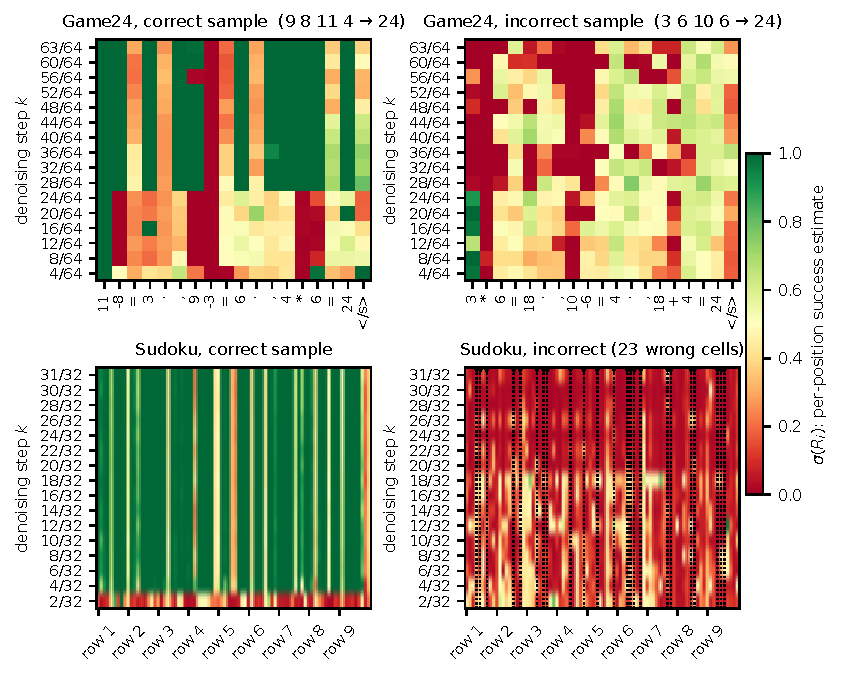
\includegraphics[width=0.58\linewidth]{figures/fig_critic_maps.pdf}
\caption{Per-position critic readings $r_{k,i}$ (colour) along the deployment-sampler trajectory (rows: denoising step $k$; columns: generated positions, labelled by the decoded token for Game24 and by Sudoku row) for one correct and one incorrect held-out sample per task. The correct samples are the median-valued correct rollout; the incorrect Game24 sample is the median-valued failed rollout and the incorrect Sudoku sample the failed rollout with the fewest wrong cells (dotted lines and markers).}
\label{fig:critic_maps}
\end{figure}

\subsubsection{1D against 2D critic over training, all tasks}
\label{app:traj}
Figure~\ref{fig:traj} extends the left panel of Figure~\ref{fig:dyn} from Game24 to the four tasks and adds the AUC of the jointly trained head. On Game24 and K\&K both heads keep up with the policy and the 2D critic's policy climbs further; on Countdown the pooled head falls behind the moving policy and its policy turns back; on Sudoku both heads keep their AUC while both policies turn back early, the 2D critic's later and from a higher peak.

\begin{figure}[!t]
\centering
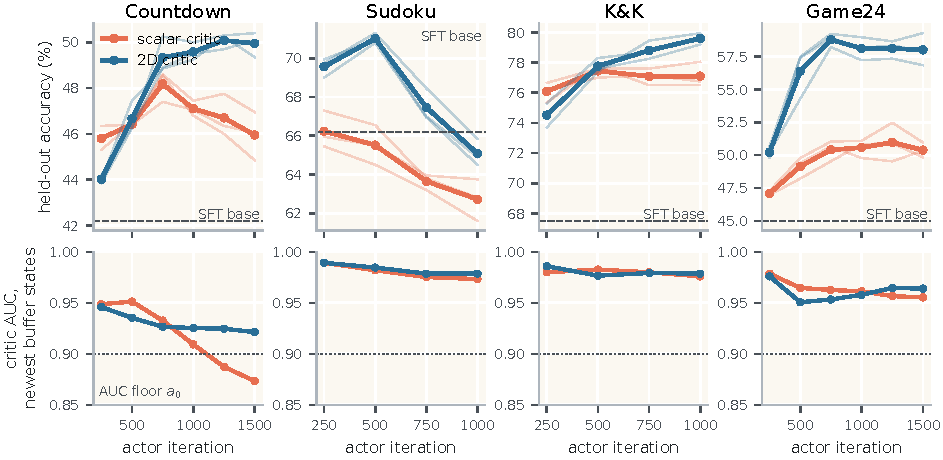
\includegraphics[width=0.85\linewidth]{figures/fig_traj.pdf}
\caption{1D against 2D critic over training: the runs of Table~\ref{tab:main}, individual runs (thin) and their mean (thick). Top: held-out accuracy (\%) at the deployment sampler of the checkpoint after that many actor iterations; dashed: the SFT base. Bottom: AUC of the jointly trained head against the outcome on the newest 256 replay-buffer states, averaged over 250-iteration windows of the training logs; dotted: the floor $a_0=0.9$ below which Algorithm~\ref{alg:jpc} gives the critic extra steps. Bottom-row curves are means over the runs. On Countdown the pooled head falls behind the moving policy and its policy turns back; on Sudoku both heads keep their AUC and the 1D critic's policy declines from the start; on Game24 and K\&K both heads keep up and the 1D critic's gain is smaller.}
\label{fig:traj}
\end{figure}

\subsubsection{The 1D and the 2D critic are interchangeable at a fixed policy}
\label{app:critic_equiv}
Table~\ref{tab:critic_equiv} compares the pre-trained 1D and 2D critics of the Table~\ref{tab:main} runs on the same states of the same policy, and their jointly trained heads on fixed probe sets. Measured this way the two critics discriminate the reward equally well, prescribe parameter updates at cosine $0.83$--$0.90$ of each other, react equally, and weakly, to a single wrong token, and their heads refit equally stably. None of the fixed-policy measurements separates the two critics: whatever distinguishes the policies they train (Figures~\ref{fig:dyn} and~\ref{fig:traj}) is not visible in either critic's value, slope or stability at a fixed policy, which is why we attribute the difference to the joint training rather than to what the critics can represent.

\begin{table}[!t]\centering\small
\caption{1D against 2D critic on the same states. Pre-trained critics unless a row says otherwise; $k$ is the denoising step of the state.}\label{tab:critic_equiv}
\footnotesize\setlength{\tabcolsep}{3pt}
\begin{tabular}{@{}p{0.35\linewidth}p{0.20\linewidth}>{\raggedright\arraybackslash}p{0.20\linewidth}>{\raggedright\arraybackslash}p{0.20\linewidth}@{}}\toprule
measurement & setting & 1D & 2D\\\midrule
Pearson correlation of the pooled value with the outcome, held-out rollouts & pre-training, Game24 $k{=}48$ / Sudoku $k{=}18$ / Countdown $k{=}14$ & 0.97 / 0.94 / 0.99 & 0.97 / 0.94 / 0.99\\
pathwise SNR of the actor's parameter gradient (Table~\ref{tab:snr} statistic) & Game24 $k{=}16$ / 24 / 32 & 0.19 / 0.17 / 0.20 & 0.18 / 0.18 / 0.15\\
half-split cosine of the actor's parameter gradient & Game24 $k{=}16$ / 24 / 32 & 0.81 / 0.78 / 0.83 & 0.81 / 0.79 / 0.70\\
cosine between the two critics' mean actor gradients & Game24 $k{=}16$ / 24 / 32 & \multicolumn{2}{l}{0.90 / 0.88 / 0.83}\\
cosine between the two critics' per-position gradient-norm profiles & Game24, real tokens & \multicolumn{2}{l}{0.94 / 0.94 / 0.94}\\
mean pairwise cosine of per-position state gradients $\partial V_\phi/\partial\rvz_{t_k}[i]$ (shared direction) & Game24 $k{=}24$ / Sudoku $k{=}12$ & 0.03 / 0.06 & 0.04 / 0.07\\
pooled $\Delta V_\phi$ (logits) for one wrong token in a successful state & Game24 $k{=}24$, re-encoded & $-0.86$ & $-0.89$\\
\quad the same, corruptions that break the answer & Game24 $k{=}24$ & $-1.76$ & $-2.04$\\
pooled $\Delta V_\phi$ for one wrong cell (never changes the decoded grid) & Sudoku $k{=}12$ & $-0.11$ & $-0.03$\\
jointly trained head: AUC on states of its own peak policy, iteration 0 $\to$ end & Game24 / Sudoku / Countdown & 0.97$\to$0.96 / 0.98$\to$0.98 / 0.90$\to$0.92 & 0.96$\to$0.96 / 0.98$\to$0.98 / 0.90$\to$0.91\\
jointly trained head: AUC on the newest buffer states, mean over training & Game24 / Sudoku / K\&K / Countdown & 0.96 / 0.98 / 0.98 / 0.92 & 0.96 / 0.98 / 0.98 / 0.93\\
actor gradient after 20 head refits: cosine to the gradient before them & Game24 $k{=}32$, buffer displaced 5\%/refit & 0.98 & 0.99\\
\bottomrule\end{tabular}\end{table}

% ---- CUT 2026-09-26 (not needed for the main narrative): State-gradient profiles of the 1D and the 2D critic ----
\iffalse
\subsubsection{State-gradient profiles of the scalar and the 2D critic}
\label{app:actor_signal}
Table~\ref{tab:actor_signal} reads the actor's instruction $g_i=\partial V_\phi/\partial y_{k,i}$ for the pre-trained scalar and 2D Game24 critics on the same 256 states of the SFT policy under the deployment chain, restricted to the real tokens of each response (18 of 64 generated positions on average). Top-10\% share: fraction of $\sum_i\|g_i\|^2$ on the 10\% of positions with the largest norm (uniform baseline $0.11$). Spearman: rank correlation across positions between $\|g_i\|$ and the undecidedness of position $i$, the negative margin between the decoder's top two logits at $\hat x_{k-1,i}$. The two critics' profiles agree at cosine $0.94$ (Spearman $0.90$) at every step: the order of head and mean does not change where the signal lands on the state, so the 2D critic's gain in Table~\ref{tab:main} is not a redistribution of the actor's signal over positions. For both critics about three quarters of the squared norm of $\nabla_{\theta}V_\phi$ flows through the estimate channel $\hat x_{k-1}$ of~(\ref{eq:chainrule}) rather than through the re-noised state, which supports reading the estimate (Section~\ref{sec:critic}).
\begin{table}[H]\centering\small
\caption{Per-position actor signal on Game24 (real tokens; mean over 256 states).}\label{tab:actor_signal}
\begin{tabular}{@{}llccc@{}}\toprule
 & & $k=16$ & $k=24$ & $k=32$\\\midrule
\multirow{2}{*}{top-10\% share of $\sum_i\|g_i\|^2$} & scalar critic & 0.43 & 0.45 & 0.45\\
 & 2D critic & 0.44 & 0.45 & 0.45\\\midrule
\multirow{2}{*}{Spearman$(\|g_i\|,\ \text{undecidedness})$} & scalar critic & 0.61 & 0.60 & 0.59\\
 & 2D critic & 0.64 & 0.64 & 0.60\\\midrule
\multirow{2}{*}{share of the signal through the estimate channel $\hat x_{k-1}$} & scalar critic & 0.79 & 0.79 & 0.79\\
 & 2D critic & 0.77 & 0.77 & 0.77\\\midrule
cosine of the two critics' $\|g_i\|$ profiles & & 0.94 & 0.94 & 0.94\\\bottomrule\end{tabular}\end{table}

\fi


% ---- CUT 2026-09-26 (not needed for the main narrative): Exchanging the critics (late exchanges) ----
\iffalse
\subsubsection{Exchanging the critics}
\label{app:swap_late}
In the right panel of Figure~\ref{fig:dyn} the scalar critic's policy handed to the 2D critic at iteration 250 climbs to within a point of the run that had the 2D critic throughout, and the 2D critic's policy handed to the scalar critic stops where the scalar runs stop; the critic in charge for the rest of the schedule decides where the run ends, not the policy it starts from.
Table~\ref{tab:swap} gives the values behind the right panel of Figure~\ref{fig:dyn}: a run of each recipe is stopped at iteration 250 and continued for the rest of the same schedule (cosine $0.94\times10^{-6}\to10^{-7}$ over the remaining 1{,}250 iterations) with its own critic or with the other recipe's pre-trained critic, whose head is refit from iteration 250 on as in Algorithm~\ref{alg:jpc}. \begin{table}[H]\centering\small
\caption{Exchanging the critics on Game24. Each cell is the held-out accuracy (\%) at the deployment sampler after that many actor iterations in total.}\label{tab:swap}
\begin{tabular}{@{}llcccccc@{}}\toprule
policy at iteration 250 & critic from 250 on & 250 & 500 & 750 & 1000 & 1250 & 1500 \\\midrule
trained with the scalar critic & scalar (unchanged) & 47.7 & 49.8 & 51.6 & 49.8 & 49.9 & 50.8 \\
 & 2D (exchanged) & 47.7 & 51.3 & 51.5 & 54.2 & 55.8 & 56.4 \\\midrule
trained with the 2D critic & 2D (unchanged) & 49.8 & 52.3 & 52.4 & 56.1 & 56.7 & 57.3 \\
 & scalar (exchanged) & 49.8 & 51.7 & 51.8 & 50.1 & 50.1 & 51.3 \\
\bottomrule\end{tabular}\end{table}
The exchange above is made while the policy is still moving. Table~\ref{tab:swap_late} makes it at iteration 750 instead, from the 2D-critic run of Table~\ref{tab:main} at iteration 750, continuing for 750 more iterations at a learning rate that has already decayed (cosine $5\times10^{-7}\to10^{-7}$) with either the 2D or the scalar critic, pre-trained and refit as in Algorithm~\ref{alg:jpc}. The two continuations are indistinguishable and both stay within two points of their starting point: once the policy has reached its plateau and the step size is small, the pooled value is no longer a shortcut the actor can take, and the field has nothing left to add. The difference between the two critics is made while the policy moves.
\begin{table}[H]\centering\small
\caption{Late exchange on Game24. The 2D-critic policy at iteration 750 (held-out $58.2$) is continued for 750 more iterations with either critic; held-out accuracy (\%) at the deployment sampler after that many further iterations.}\label{tab:swap_late}
\begin{tabular}{@{}lccc@{}}\toprule
critic from iteration 750 on & +250 & +500 & +750\\\midrule
2D & 57.5 & 56.7 & 57.3\\
scalar & 57.0 & 56.4 & 56.2\\
\bottomrule\end{tabular}\end{table}

\fi


\subsubsection{Frozen versus joint critic}
\label{app:frozen}
The right panel of Table~\ref{tab:critic_design} shows the exploit directly on Game24: the recipe of Algorithm~\ref{alg:jpc} with the pre-trained 2D critic held fixed. The pathwise update first helps, then the actor finds the critic's blind spots: the critic's value on the training batch climbs from about $3$ logits at iteration 250 to over $80$ by 1500 while the true success rate of the same batch falls from $78\%$ to $0\%$, and the held-out accuracy collapses. The identical run with the head refit after every actor step (Table~\ref{tab:main}) keeps the critic's value in the calibrated range. Increasing the frozen critic's quality (more pre-training rollouts, the 2D form) does not change this: whatever the critic is, the actor exploits it within a few hundred updates unless the critic is refreshed on the actor's own states.

% ---- CUT 2026-09-26 (not needed for the main narrative): Which parts of the critic are trained, and from where ----
\iffalse
\subsubsection{Which parts of the critic are trained, and from where}
\label{app:critic_training}
Table~\ref{tab:critic_training} separates the two choices behind the critic of Algorithm~\ref{alg:jpc}: that its network starts as a copy of the denoiser, and that during RL only its head is refit. All four runs share the frozen text encoder, the actor, the critic architecture, the pre-training rollouts and epochs, and the head refit of Algorithm~\ref{alg:jpc}; they differ only in how the critic's network is initialised before pre-training and in whether it receives gradients during RL (learning rate $10^{-5}$, that of pre-training). Training the copy during RL costs eight points and its gain does not carry to the cheap chain ($33.6$ against $35.4$ for the base). A randomly initialised network, pre-trained on the same rollouts, reads the outcome only weakly (Table~\ref{tab:critic_design}) and takes the policy below the base. Training it during RL then acts as a stabiliser and not as a remedy: with its network frozen the weak critic is exploited to collapse, the same collapse as the frozen critic in the right panel of Table~\ref{tab:critic_design}, and with its network trained the policy settles twelve points under the base.
\begin{table}[H]\centering\small
\caption{How the critic's network is obtained and trained (Game24, Algorithm~\ref{alg:jpc} otherwise). Each cell is the held-out accuracy (\%) at the deployment sampler after that many actor iterations; the base is $45.0$. The random initialisation resets every attention, feed-forward and embedding weight of the network; its few learned prefix tokens and normalisation gains keep their values. Blue: the critic of Algorithm~\ref{alg:jpc}.}\label{tab:critic_training}
\begin{tabular}{@{}llcccccc@{}}\toprule
network before pre-training & network during RL & 250 & 500 & 750 & 1000 & 1250 & 1500 \\\midrule
\hl{copy of the denoiser} & \hl{frozen} & 49.8 & 57.2 & 58.2 & 56.2 & 56.5 & 57.5 \\
copy of the denoiser & trained & 47.2 & 49.7 & 47.3 & 47.4 & 48.8 & 49.3 \\
random & trained & 39.2 & 35.4 & 34.2 & 33.5 & 33.4 & 33.4 \\
random & frozen & 37.9 & 24.2 & \phantom{0}1.4 & \phantom{0}0.8 & \phantom{0}2.6 & \phantom{0}4.1 \\
\bottomrule\end{tabular}\end{table}

\fi


% ---- CUT 2026-09-26 (not needed for the main narrative): Ablations: full checkpoint trajectories ----
\iffalse
\subsubsection{Ablations: full checkpoint trajectories}
\label{app:needs_full}
Table~\ref{tab:needs_full} gives every evaluated checkpoint behind Table~\ref{tab:needs}. The probability objective and minimum pooling stay below the reference at every checkpoint, and training under the cheap chain stays below it at deployment throughout. The five-step buffer of block B was also run on Countdown, where the outcome is not readable before the middle of the chain (held-out AUC $0.64$ at steps 8--24 against $0.90$ at step 40): there it costs over two points against the single-step buffer of Algorithm~\ref{alg:jpc} with the same pre-trained critic ($47.9$ against $50.2$ at the deployment sampler), which is why the recipe refits at $k_{\rm hi}$.

The per-position loss term is the one choice whose ablation depends on the task. On Game24, refitting the 2D critic with the pooled term of~(\ref{eq:critic2d_loss}) alone changes nothing. On Countdown, where the scalar critic's head falls behind its policy (Appendix~\ref{app:traj}), the same ablation removes the 2D critic's advantage (block A): the runs peak at about $47$ and end at about $45$, against end values of about $50$ with both terms and $45.4$ for the scalar critic. Its head also degrades as the scalar head does: the in-sample AUC of the last 250 iterations is $0.88$ against $0.91$--$0.93$ with both terms, and the AUC check fires in $20$--$21$ of the last $25$ tests against $0$--$8$. More refit does not help the scalar critic either. With $m_{\rm c}{=}8$ head steps per actor step in place of $2$, the scalar-critic runs end at $42$--$46$, no better than with two steps, and the head's in-sample AUC falls faster ($0.83$ in the last 250 iterations, the check firing every time). The scalar critic's stall on Countdown is thus not a matter of refit budget, and the order of head and mean alone does not remove it; what does is fitting every reading to the outcome, the constraint Section~\ref{sec:jpc_2d} introduces the second term for.
\begin{table}[H]
\centering\small
\caption{Full checkpoint trajectories of the ablations of Table~\ref{tab:needs}. Each cell is the held-out accuracy (\%) at the deployment sampler of the checkpoint saved after that many actor iterations; \emph{best} is the highest cell of the row (for rows that average several runs, the mean of their per-run maxima); the SFT base is $45.0$. Rows are single runs unless the number of runs is given, and then the cells are means over them. Blocks A--C are the recipe versions of Appendix~\ref{app:details}; block A stands behind rows 1--2 of Table~\ref{tab:needs} and block C behind row 3; reference rows are means over three runs. Blue: recommended variant; bold: the highest cell of the row.}
\label{tab:needs_full}
\scriptsize\setlength{\tabcolsep}{3pt}
\begin{tabular}{@{}>{\raggedright\arraybackslash}p{0.17\linewidth}>{\raggedright\arraybackslash}p{0.34\linewidth}cccccc|c@{}}
\toprule
choice it tests & variant & \multicolumn{6}{c}{accuracy after $n$ actor iterations} & best \\
 & & $n{=}250$ & 500 & 750 & 1000 & 1250 & 1500 & \\
\midrule
\multicolumn{9}{@{}l}{\emph{A. Algorithm~\ref{alg:jpc} (single-step buffer, both loss terms, AUC check, cosine decay)}}\\
 & \hl{reference (3 seeds)} & 50.2 & 56.4 & 58.8 & 58.1 & 58.1 & 58.0 & \textbf{58.8} \\
Section~\ref{sec:pathwise}, objective & actor ascends $\mathrm{sig}(V_\phi)$ instead of $V_\phi$ & \ABp{1} & \ABp{2} & \ABp{3} & \ABp{4} & \ABp{5} & \ABp{6} & \ABp{7} \\
Section~\ref{sec:jpc_2d}, pooling & actor ascends $\min_iR_{k,i}$ instead of the mean & \ABm{1} & \ABm{2} & \ABm{3} & \ABm{4} & \ABm{5} & \ABm{6} & \ABm{7} \\
 & \emph{Countdown:} reference (3 seeds; base $42.2$) & 44.0 & 46.6 & 49.3 & 49.6 & 50.1 & 50.0 & 50.2 \\
Section~\ref{sec:pathwise}, objective & \emph{Countdown:} actor ascends $\mathrm{sig}(V_\phi)$ & \ABcp{1} & \ABcp{2} & \ABcp{3} & \ABcp{4} & \ABcp{5} & \ABcp{6} & \ABcp{7} \\
 & \emph{Countdown:} reference (2 runs) & 44.2 & 47.3 & 49.8 & 49.9 & 49.4 & 50.2 & 50.4 \\
Section~\ref{sec:jpc_2d}, supervision & \emph{Countdown:} pooled loss term only (2 runs) & 44.2 & 44.0 & 45.8 & 46.4 & 45.8 & 44.8 & 46.9 \\
 & \emph{Countdown:} scalar critic, $m_{\rm c}{=}2$ (3 runs) & 45.8 & 46.4 & 48.2 & 47.1 & 46.7 & 45.9 & 48.2 \\
Section~\ref{sec:joint}, critic ahead of actor & \emph{Countdown:} scalar critic, $m_{\rm c}{=}8$ (2 runs) & 42.8 & 44.5 & 43.8 & 44.5 & 44.1 & 43.8 & 44.9 \\
\midrule
\midrule
\multicolumn{9}{@{}l}{\emph{C. 1000 iterations, constant learning rate $10^{-6}$, five-step buffer}}\\
 & reference & 48.7 & 50.9 & 53.0 & 56.4 & --- & --- & 56.4 \\
Section~\ref{sec:joint}, critic must move & critic frozen after pre-training & 48.4 & 48.0 & \phantom{0}2.1 & \phantom{0}0.3 & --- & --- & 48.4 \\
Section~\ref{sec:joint}, critic ahead of actor & $m_{\rm c}{=}1$ head step per actor step & 48.0 & 51.7 & 48.6 & 51.1 & --- & --- & 51.7 \\
 & $m_{\rm c}{=}8$ & 47.0 & 52.3 & 54.7 & 55.2 & --- & --- & 55.2 \\
Section~\ref{sec:joint}, staleness & buffer $N_{\mathcal B}{=}4$k instead of 16k & 47.8 & 50.1 & 52.6 & 56.4 & --- & --- & 56.4 \\
Section~\ref{sec:joint}, one chain & trained under $\gamma4$@16, read at $\gamma56$@64 & 44.7 & 44.3 & 41.5 & 47.0 & --- & --- & 47.0 \\
 & \quad the same run read at $\gamma4$@16 (base $35.4$) & 35.1 & 38.7 & 41.3 & 42.5 & --- & --- & 42.5 \\
\bottomrule
\end{tabular}
\end{table}

\fi


\subsubsection{Training dynamics on Countdown and K\&K}
\label{app:dynamics}
Figure~\ref{fig:dynamics_cd_kk} shows the Algorithm~\ref{alg:jpc} runs with the 2D critic on the two tasks not covered by Figure~\ref{fig:dyn}. On Countdown the held-out accuracy rises for about 750 iterations and then holds while the replay-buffer success rate keeps climbing: the training batch keeps improving after the held-out set has levelled off. On K\&K the held-out accuracy rises monotonically and is still at its peak when the schedule ends; its buffer success rate and critic value rise together over the whole run.

% ---- CUT 2026-09-26 (not needed for the main narrative): Figure with the Game24 loop check ----
\iffalse
\begin{figure}[H]
\centering
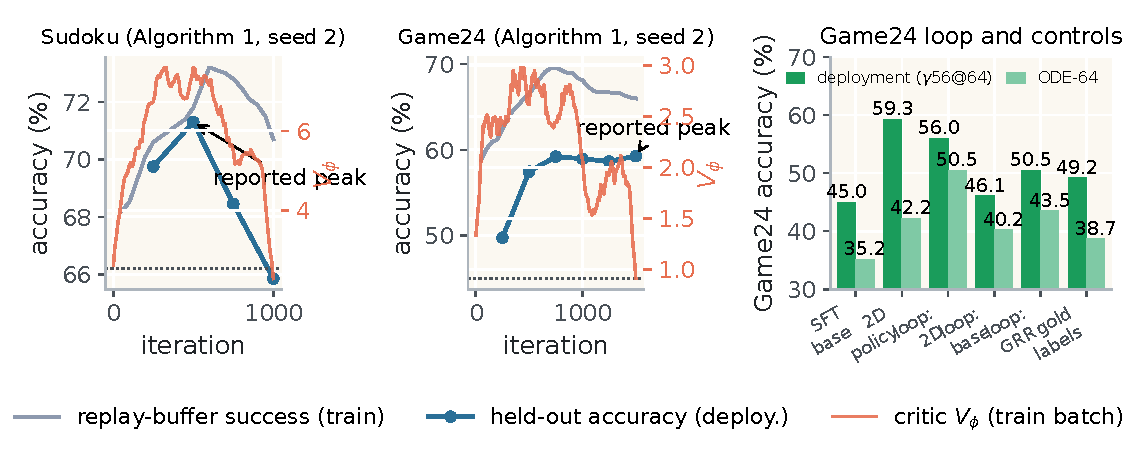
\includegraphics[width=\linewidth]{figures/fig_dynamics_loop.pdf}
\caption{Left, middle: two Algorithm~\ref{alg:jpc} runs (2D critic, cosine $10^{-6}\!\to\!10^{-7}$): replay-buffer success (grey), critic value on the training batch (red) and held-out accuracy at the deployment sampler (blue).Right: the Game24 rounds and their controls at the deployment and ODE-64 samplers (base; 2D-critic policy; four plain rounds from that policy, from the base, from the GRPO policy, and on gold labels), the check of Appendix~\ref{app:g24_loop}.}
\label{fig:curves}
\end{figure}
\fi

\begin{figure}[H]
\centering
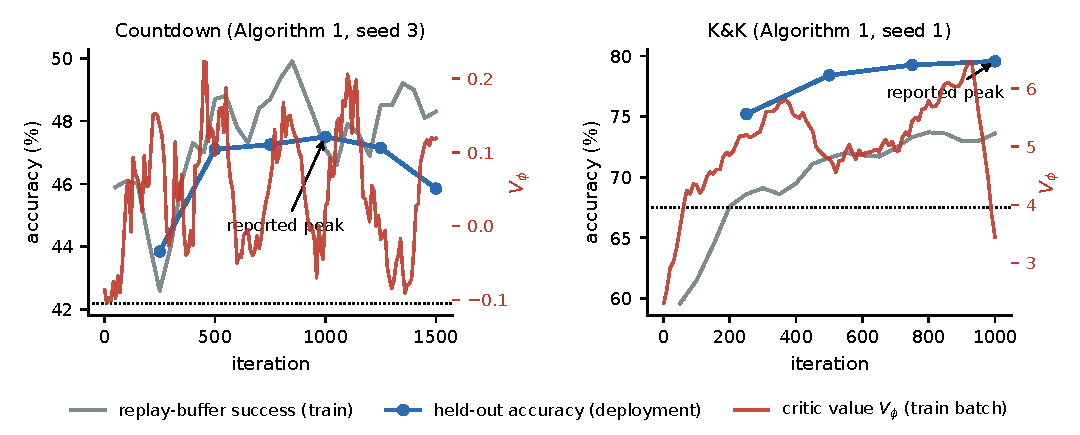
\includegraphics[width=0.85\linewidth]{figures/fig_dynamics_cd_kk.pdf}
\caption{Training dynamics of Algorithm~\ref{alg:jpc} (2D critic) on Countdown (left) and K\&K (right): held-out accuracy at the deployment sampler per checkpoint (blue), replay-buffer success rate (grey), and the critic's value on the training batch (red, right axis); dotted line: SFT base.}
\label{fig:dynamics_cd_kk}
\end{figure}

\subsection{The loop}
This group stands behind Table~\ref{tab:loop}: every round of every loop with its controls, and the critic-guided sampler that draws the later Countdown rounds.

\subsubsection{The loop in full: rounds, controls and the guided sampler}
\label{app:loop_full}
Table~\ref{tab:loop_full} gives every round behind Table~\ref{tab:loop} with the pool's coverage and the controls. On Countdown and K\&K the rounds lift the cheap sampler by 17 to 35 points from every start, RL or not. On K\&K fresh puzzles give near-full coverage from any start and the rounds close the task; RL adds nothing there that the rounds do not. On Sudoku one round covers three quarters of the pool from every start and moves accuracy by at most 1.4 points at either sampler, as the gold-solution control confirms. On Countdown two plain rounds shrink coverage and give back part of the RL gain; rounds 3 and 4, drawn with the critic-guided cheap sampler, raise coverage past its start and return the deployment sampler to the RL level, 5 to 7 points above sampling plainly from the base or the \methodGRPO{} policy. Two further plain rounds continued from the round-2 model (the two control rows after round 4) leave coverage and accuracy at the round-2 level, whereas the critic-guided rounds from the same model cover about six thousand more problems and recover $4.5$--$5.9$ points at deployment; the recovery is therefore due to the critic-guided pools, not to the additional rounds. 

% Table~\ref{tab:guided} isolates the guided sampler on the first $5{,}000$ pool problems with the loop's starting policy and its jointly trained critic at $\gamma4$@16: pruning four trajectories at random changes nothing; pruning them by the critic's minimum reading~(\ref{eq:minscore}) doubles the acceptance rate and raises coverage by a third, and the push~(\ref{eq:guide}) adds to both.

\begin{table}[H]
\centering\small
\caption{The amortization loop, held-out accuracy (\%) at three samplers. Each block is one task: the SFT base, the 2D-critic policy the loop starts from, the model at the end of each round of Algorithm~\ref{alg:loop} (Countdown: all four rounds; K\&K: first and last of five; Sudoku: its one round), and, indented, the controls at their last round, which run the same rounds without a critic from the SFT base, from the \methodGRPO{} policy, and on the gold derivations of the same pool, and, for Countdown, two further plain rounds continued from the round-2 model. \emph{Covered}: pool problems (of 50k) with at least one verified sample in that round. Game24 has no pool of unlabelled problems. Sudoku's cheap sampler is $\gamma14$@16 and its deployment sampler $\gamma28$@32. Bold: the last round of each loop where it is over 1.0 point above the start.}
\label{tab:loop_full}
\setlength{\tabcolsep}{4.5pt}
\begin{tabular}{@{}llcccc@{}}
\toprule
 & pool sampler & covered & 16-step sampler & ODE-64 & deployment \\
\midrule
\multicolumn{6}{@{}l}{\emph{Countdown}}\\
SFT base & & & 23.8 & 28.5 & 42.8 \\
2D-critic policy (start) & & & 24.3 & 34.8 & 50.5 \\
round 1 & deployment sampler & 35.1k & 37.9 & 42.4 & 45.8 \\
round 2 & deployment sampler & 31.2k & 40.8 & 42.6 & 46.0 \\
round 3 & critic-guided, $\gamma4$@16 & 37.2k & \OURScdthreeg & \OURScdthreeo & \OURScdthree \\
round 4 & critic-guided, $\gamma4$@16 & 37.8k & \textbf{\OURScdg} & \textbf{\OURScdo} & \OURScd \\
\quad plain round 3 (control) & deployment sampler & 31.2k & 41.1 & 43.7 & 45.5 \\
\quad plain round 4 (control) & deployment sampler & 31.3k & 41.1 & 43.4 & 45.5 \\
\quad control: from the SFT base & deployment sampler & 31.2k & 42.7 & 44.5 & 46.4 \\
\quad control: from \methodGRPO{} & deployment sampler & 30.9k & 41.1 & 42.9 & 44.7 \\
\quad control: gold derivations & (labels) & 50.0k & 22.5 & 26.4 & 40.8 \\
\midrule
\multicolumn{6}{@{}l}{\emph{K\&K}}\\
SFT base & & & 58.6 & 57.5 & 68.2 \\
2D-critic policy (start) & & & 68.8 & 69.7 & 79.8 \\
round 1 & deployment sampler & 41.1k & 73.4 & 76.6 & 82.1 \\
round 5 & deployment sampler & 48.8k & \textbf{\OURSkkg} & \textbf{\OURSkko} & \textbf{\OURSkk} \\
\quad control: from the SFT base & deployment sampler & 49.4k & 93.5 & 97.0 & 99.6 \\
\quad control: from \methodGRPO{} & deployment sampler & 48.3k & 91.7 & 94.6 & 97.9 \\
\quad control: gold labels & (labels) & 50.0k & 94.8 & 98.0 & 99.6 \\
\midrule
\multicolumn{6}{@{}l}{\emph{Sudoku}}\\
SFT base & & & 60.0 & 60.6 & 64.0 \\
2D-critic policy (start) & & & 63.4 & 65.3 & 68.9 \\
round 1 & deployment sampler & 39.3k & 63.1 & 65.4 & \textbf{70.3} \\
\quad control: from the SFT base & deployment sampler & 36.1k & 58.7 & 60.7 & 63.6 \\
\quad control: from \methodGRPO{} & deployment sampler & 39.3k & 64.2 & 67.7 & 69.6 \\
\quad control: gold solutions & (labels) & 50.0k & 63.9 & 65.2 & 69.7 \\
\bottomrule
\end{tabular}
\end{table}

% \begin{table}[H]
% \centering\small
% \caption{The critic as a search heuristic. Each row is one way of drawing samples from the Countdown 2D-critic policy the loop starts from (Table~\ref{tab:loop_full}) and its jointly trained critic at $\gamma4$@16 on the first 5{,}000 pool problems, four samples per problem: \emph{acc.}, the fraction of samples the verifier accepts; \emph{coverage}, problems (of 5{,}000) with at least one accepted sample; \emph{distinct}, distinct accepted derivations.}
% \label{tab:guided}
% \begin{tabular}{@{}lccc@{}}
% \toprule
% sampler & acc.\ (\%) & coverage & distinct \\
% \midrule
% plain & \GBa{1} & \GBa{2} & \GBa{3} \\
% best of 4 at step 8, random & \GBb{1} & \GBb{2} & \GBb{3} \\
% best of 4 at step 8, by the critic & \GBc{1} & \GBc{2} & \GBc{3} \\
% push~(\ref{eq:guide}) at every step & \GBd{1} & \GBd{2} & \GBd{3} \\
% best of 4 by the critic + push & \GBe{1} & \GBe{2} & \GBe{3} \\
% \bottomrule
% \end{tabular}
% \end{table}

% ---- CUT 2026-09-26 (not needed for the main narrative): Cheap samplers after the loop ----
\iffalse
\subsubsection{Cheap samplers after the loop}
\label{app:samplers}
Table~\ref{tab:samplers} reads one 2D-critic checkpoint per task and its loop across sampler cost. RL alone moves Countdown's cheap samplers little ($+0.5$ at $\gamma4$@16 against $+7.7$ at deployment), whereas on K\&K and Sudoku the RL gain carries to every sampler. One loop moves the rest: after it, the 16-step sampler reaches or passes the accuracy the 64-step deployment sampler had before RL on Countdown and K\&K ($\OURScdg$ vs $42.8$, $\OURSkkg$ vs $68.2$), and on K\&K it passes the deployment accuracy of the RL policy itself ($\OURSkkg$ vs $79.8$). Sudoku, whose loop is null, moves by at most 1.4 points at any sampler; Game24 has no loop (Appendix~\ref{app:g24_loop}).

\begin{table}[H]\centering\small
\caption{The loop moves what the policy can do to the cheap samplers. Held-out accuracy (\%) at samplers of increasing cost: the SFT base, the 2D-critic policy and the model after the loop (final round). $^\dagger$On Sudoku this column is $\gamma14$@16 and the deployment column is $\gamma28$@32. Bold: the best row of each block; blue: recommended variant.}\label{tab:samplers}
\begin{tabular}{@{}llcccc@{}}\toprule
 & & $\gamma4$@16 & $\gamma28$@32$^\dagger$ & ODE-64 & deployment\\\midrule
\multirow{3}{*}{Countdown} & SFT base & 23.8 & 38.1 & 28.5 & 42.8\\
 & 2D-critic policy & 24.3 & 43.9 & 34.8 & 50.5\\
 & \hl{+ loop} & \textbf{45.6} & \textbf{51.1} & \textbf{47.8} & \textbf{51.4}\\\midrule
\multirow{3}{*}{Sudoku} & SFT base & 52.5 & 60.0 & 60.6 & 64.0\\
 & 2D-critic policy & \textbf{54.2} & \textbf{63.4} & 65.3 & 68.9\\
 & \hl{+ loop} & 53.7 & 63.1 & \textbf{65.4} & \textbf{70.3}\\\midrule
\multirow{3}{*}{K\&K} & SFT base & 58.6 & 66.3 & 57.5 & 68.2\\
 & 2D-critic policy & 68.8 & 76.3 & 69.7 & 79.8\\
 & \hl{+ loop} & \textbf{93.8} & \textbf{97.9} & \textbf{95.7} & \textbf{99.1}\\\midrule
\multirow{2}{*}{Game24} & SFT base & 35.6 & 43.5 & 36.2 & 44.0\\
 & 2D-critic policy & \textbf{38.9} & \textbf{54.2} & \textbf{43.5} & \textbf{59.6}\\
\bottomrule\end{tabular}\end{table}

\fi


% ---- CUT 2026-09-26 (not needed for the main narrative): Countdown loop round by round ----
\iffalse
\subsubsection{Countdown loop round by round}
\label{app:cd_loop}
Table~\ref{tab:cd_loop} lists every round of the Countdown loop at all four samplers, together with three of the controls of Table~\ref{tab:loop_full}, which run the same four rounds from the SFT base, from the GRPO policy, and from the 2D policy on the gold labels of the same pools. Three regularities are visible. (i) The loop transfers the policy's ability to the cheap samplers at once: one round takes the ODE sampler from $34.8$ to $42.4$ and $\gamma4$@16 from $24.3$ to $37.9$ while the deployment sampler gives back nearly 5 points. (ii) Plain self-sampling loses ground at the deployment sampler ($50.5\to45.8\to46.0$) and the pool's coverage shrinks (35.1k to 31.2k solved problems). (iii) Sampling the pool with the jointly trained 2D critic (best-of-4 pruning at the midpoint of the 16-step chain plus gradient guidance, Appendix~\ref{app:details}) restores coverage and lifts the deployment sampler ($\OURScdthree$ after round 3, $\OURScd$ after round 4). The plain chains from the base and from the GRPO policy show the first two regularities and stop at $45$--$46$; the gold-label chain falls from $50.5$ to $45.5$ in its first round and drifts to $40.8$ by round 4 (ODE-64 from $34.8$ to $26.4$): fine-tuning the RL policy on gold derivations undoes part of what RL changed rather than adding to it.

\begin{table}[H]\centering\small
\caption{Countdown amortisation loop, held-out accuracy at the end of each round (20 epochs of fine-tuning per round; verifier-accepted sequences and distinct problems in each pool). From top: loop from the 2D-critic policy (Table~\ref{tab:loop}); from the SFT base with no RL; from the GRPO policy; from the 2D-critic policy on the gold labels of the same pools.}\label{tab:cd_loop}
\scriptsize\setlength{\tabcolsep}{2.5pt}
\begin{tabular}{@{}llcccc@{}}\toprule
round & pool & ODE-64 & $\gamma4$@16 & $\gamma28$@32 & $\gamma56$@64\\\midrule
SFT base (epoch 60) & & 28.5 & 23.8 & 38.1 & 42.8\\
\methodSVGTwoD{} policy (start) & & 34.8 & 24.3 & 43.9 & 50.5\\
round 1 & deployment sampler, 91.9k sequences / 35.1k problems & 42.4 & 37.9 & 45.0 & 45.8\\
round 2 & deployment sampler, 57.4k / 31.2k & 42.6 & 40.8 & 45.3 & 46.0\\
round 3 & 2D-critic-guided sampler, \OURSpoolthree & \OURScdthreeo & \OURScdthreeg & \OURScdthreet & \OURScdthree\\
round 4 & 2D-critic-guided sampler, \OURSpoolfour & \OURScdo & \OURScdg & \OURScdt & \OURScd\\\midrule
no-RL round 1 & deployment sampler, 82.4k / 34.2k & 40.1 & 34.4 & 44.8 & 46.6\\
no-RL round 2 & 59.1k / 30.8k & 42.0 & 39.9 & 45.5 & 46.8\\
no-RL round 3 & 52.2k / 30.8k & 43.7 & 43.3 & 45.8 & 46.1\\
no-RL round 4 & 48.5k / 31.2k & 44.5 & 42.7 & 46.3 & 46.4\\\midrule
GRPO policy (start) & & 29.5 & 23.7 & 40.1 & 43.0\\
GRPO round 1 & deployment sampler, 82.7k / 34.1k & 42.7 & 39.0 & 44.8 & 46.0\\
GRPO round 2 & 58.3k / 30.5k & 43.0 & 39.8 & 45.7 & 47.1\\
GRPO round 3 & 51.3k / 30.4k & 45.2 & 41.2 & 45.7 & 47.1\\
GRPO round 4 & 47.2k / 30.9k & 42.9 & 41.1 & 44.2 & 44.7\\\midrule
gold round 1 & gold derivations, 50k / 50k & 28.2 & 24.6 & 40.2 & 45.5\\
gold round 2 & & 27.1 & 23.5 & 40.1 & 42.0\\
gold round 3 & & 25.8 & 23.2 & 40.4 & 41.0\\
gold round 4 & & 26.4 & 22.5 & 37.6 & 40.8\\\bottomrule\end{tabular}\end{table}

\fi


% ---- CUT 2026-09-26 (not needed for the main narrative): Game24: why there is no loop row ----
\iffalse
\subsubsection{Game24: why there is no loop row}
\label{app:g24_loop}
Game24 is split by number set (Appendix~\ref{app:datasets}): every solvable set is either a training set or a held-out set, so there is no pool of unlabelled problems the policy has not trained on, which is what a round of Algorithm~\ref{alg:loop} needs. Table~\ref{tab:g24_loop} shows what happens when the rounds are run regardless, on the 4{,}693 other orderings of the 1{,}076 training sets, from the 2D-critic policy and from the three control starting points. The starting policy already solves $81\%$ of that pool, so a round mostly re-fits derivations of sets it knows. Read the deployment column against the cheap-sampler columns: the rounds move the ODE and 16-step samplers up by 7 to 11 points, as on the other tasks, while the deployment sampler loses about 3 points in the first round and then holds. Sampling rounds 3--4 with the critic-guided cheap chain of Appendix~\ref{app:loop}, the recipe of the Countdown loop, raises the pool's coverage a little further and lowers every held-out number: the extra accepted derivations are more of the same sets. The gold-label control isolates the cost: fine-tuning the same policy on the gold derivations of the same prompts loses about 10 points at deployment and lowers the cheap samplers by 2 to 5 points, where the self-samples raise them by 7 to 11. What the rounds cost is the supervised fitting of training-set derivations, the effect that already limits the supervised epochs on this task (Appendix~\ref{app:g24_sft}); what they give is the transfer across samplers that the self-samples carry and the gold derivations do not. From the SFT base and from the GRPO policy the rounds gain 2 to 3 points at deployment and 3 to 6 at ODE-64. None of this is the loop of Appendix~\ref{app:loop}, whose gain comes from covering problems the policy does not yet solve, so Table~\ref{tab:loop} carries no Game24 entry.
\begin{table}[H]\centering\small
\caption{Rounds of Algorithm~\ref{alg:loop} on Game24's re-ordered training sets, held-out accuracy (\%) at the end of each round (8 epochs of fine-tuning per round). \emph{Covered}: pool problems with at least one verified sample. From top: from the 2D-critic policy (final checkpoint) with plain deployment-chain sampling, then the same chain continued from round 2 with critic-guided sampling in rounds 3--4; from the SFT base; from the GRPO policy; from the 2D-critic policy on the gold derivations of the same pool.}\label{tab:g24_loop}
\scriptsize\setlength{\tabcolsep}{4pt}
\begin{tabular}{@{}llccc@{}}\toprule
start / round & covered & $\gamma56$@64 & ODE-64 & $\gamma4$@16\\\midrule
\methodSVGTwoD{} policy (start) & & 59.6 & 43.5 & 38.9\\
round 1, plain & 3.79k / 4.69k & 56.8 & 46.9 & 44.2\\
round 2, plain & 3.54k & 56.4 & 49.1 & 48.2\\
round 3, plain & 3.58k & 56.5 & 49.1 & 47.9\\
round 4, plain & 3.64k & 57.0 & 50.5 & 50.2\\
round 3, critic-guided (from round 2) & 3.96k & 55.9 & 48.1 & 48.1\\
round 4, critic-guided & 3.95k & 51.2 & 47.1 & 45.9\\\midrule
SFT base (start) & & 44.0 & 36.2 & 35.6\\
rounds 1--4, plain & & 45.2 / 44.5 / 44.6 / 46.0 & 37.1 / 37.5 / 38.5 / 38.9 & 37.1 / 36.9 / 36.5 / 39.2\\\midrule
GRPO policy (start) & & 48.5 & 37.4 & 36.6\\
rounds 1--4, plain & & 49.4 / 48.5 / 51.7 / 51.2 & 40.0 / 40.9 / 43.1 / 43.2 & 40.5 / 40.6 / 39.6 / 42.1\\\midrule
gold derivations, rounds 1--4 & 4.69k & 54.0 / 50.4 / 49.5 / 48.8 & 38.9 / 38.4 / 39.6 / 39.0 & 39.2 / 36.9 / 36.5 / 36.5\\
\bottomrule\end{tabular}\end{table}

\fi


% ---- CUT 2026-09-26 (not needed for the main narrative): Sampler sweep on the Countdown base model ----
\iffalse
\subsubsection{Sampler sweep on the Countdown base model}
\label{app:sampler_sweep}
Table~\ref{tab:sampler_sweep} records the held-out accuracy of the Countdown SFT model under the samplers we swept before fixing the four reporting samplers. Two regularities hold on every task we tried: at a fixed number of steps $K$ the best $\gamma$ is the one that keeps the per-step retention $\alpha_k$ near $0.125$ (so $\gamma\approx K\cdot0.875$: $\gamma4$@16 is deliberately \emph{below} this and is the cheap sampler; $\gamma14$@16, $\gamma28$@32, $\gamma56$@64 and $\gamma112$@128 are on it), and at that retention more steps keep helping with diminishing returns ($38.1\to42.8\to44.0$ from 32 to 64 to 128 steps). The deployment sampler $\gamma56$@64 is the last point at which the rollout cost is acceptable for RL (64 network evaluations per sample, one of which is recomputed with gradients).

\begin{table}[H]\centering\small
\caption{Countdown held-out accuracy of the SFT model under different samplers (classifier-free guidance 2 unless stated). Left: the base checkpoint used in the paper (epoch 60). Right: an earlier checkpoint (epoch 42) on which the wider grid was run, evaluated on the full held-out set.}\label{tab:sampler_sweep}
\resizebox{\linewidth}{!}{%
\begin{tabular}{@{}lc@{\qquad}lc@{}}\toprule
sampler (epoch 60) & acc. & sampler (epoch 42) & acc.\\\midrule
ODE, 64 steps & 28.5 & ODE, 64 / 128 steps & 23.4 / 24.6\\
$\gamma4$@16 & 23.8 & $\gamma4$@16 / $\gamma14$@16 & 19.9 / 24.1\\
$\gamma28$@32 & 38.1 & $\gamma20$@32 / $\gamma28$@32 / $\gamma28$@32 (guidance 3) & 28.4 / 31.6 / 30.2\\
$\gamma56$@64 (deployment) & 42.8 & $\gamma48$@64 / $\gamma56$@64 / $\gamma56$@64 (guidance 1.5) & 33.8 / 35.0 / 34.9\\
$\gamma112$@128 & 44.0 & $\gamma112$@128 & 37.4\\\bottomrule\end{tabular}}\end{table}


\fi

